\chapter{Omitted variable bias: COMING SOON}
\label{ch-omitted-var-bias}

Recall our notation defined in Chapter \ref{ch-conventions}:
\beq
E[\rva]=\av{\rva}
\eeq


\beq
cov(\rva, \rvb)= \av{\rva, \rvb}=
\av{\rva\rvb}-\av{\rva}\av{\rvb}
\eeq

\beq
\s_\rva= \sqrt{\av{\rva,\rva}}
\eeq

\beq
corr(\rva, \rvb) = \rho_{\rva, \rvb}=
\frac{\av{\rva,\rvb}}{\sqrt{\av{\rva,\rva}
\av{\rvb,\rvb}}}
\leq 1
\eeq

\beq
\partial_\rvb\rva(\rvx)=
\frac{\av{\rvb, \rva}^{|\rvx-\rvb}}{\av{\rvb, \rvb}^{|\rvx-\rvb}}
=
\rho_{\rva, \rvb}^{|\rvx-\rvb}
\frac{\s_\rva^{|\rvx-\rvb}}
{\s_\rvb^{|\rvx-\rvb}}
\eeq

\begin{figure}[h!]
$$
\begin{array}{cc}
\xymatrix{
&\rvu\ar@{-->}[ldd]_{\alp'}
\ar@{-->}[rdd]^{\beta'}
\\
&\rvx
\ar[ld]^\alp
\ar[rd]_\beta
\\
\rvd\ar[rr]_\delta
&&\rvy
}
&
\xymatrix{
&\rvx
\ar[ld]^\alp
\ar[rd]_\beta
\\
A_\rvu\rvd\ar[rr]_\delta
&&A_\rvu\rvy
}
\\
(a)&(b)
\end{array}
$$
\caption{LDEN bnets used to do PO confounder
sensitivity analysis.
Node $\rvu$
is an unobserved common cause confounder. 
The operator $A_\rvu$ in bnet $(b)$ annihilates $\rvu$ (i.e., $A_\rvu \rvu =0$)}
\label{eq-ovb-sen-ana}
\end{figure}

Consider the LDEN bnets of Fig.\ref{eq-ovb-sen-ana}.
whose structure equations,
printed in blue, are as follows:

For $(a)$,
\beq
\color{blue}
\left\{
\begin{array}{l}
\rvu = \rveps_\rvu
\\ 
\rvx = \rveps_x
\\ 
\rvd = \alp\rvx +\alp'\rvu +\rveps_\rvd
\\ 
\rvy = \delta \rvd +
\beta \rvx + \beta'\rvu + \rveps_\rvy
\end{array}
\right.
\eeq

For $(b)$,
\beq
\color{blue}
\left\{
\begin{array}{l}
\rvx^S = \rveps_x^S
\\ 
\rvd^S = \alp\rvx^S +\rveps_\rvd^S
\\
\rvy^S = \delta \rvd^S +
\beta \rvx^S  + \rveps_\rvy^S
\end{array}
\right.
\eeq

\beq
A_\rvu(\rvu, \rvx, \rvd, \rvy, \rveps)=
(0, \rvx^S, \rvd^S, \rvy^S, \rveps^S)
\eeq


\beq
\boxed{
ATE-ATE|_{\beta'=0}=\frac{\beta'}{\alp'}}
\eeq

\hrule

\beq
\rvx^3_\beta = [\rvd, \rvx, \rvu]^T
\eeq

\beq
\beta^3= [\delta, \beta, \beta']^T
\eeq

\beq
\rvy = [\beta^3]^T\rvx^3_\beta + \eps_\rvy
\eeq

\beq
(J_\beta)_{i,j} =
\pder{(\rvx_\beta)_i}{(\rvx_\beta)_j}
\eeq

\beq
\beta^3=
(J^T_\beta)^{-1}\nabla_{\rvx^3}\rvy
\eeq

\beq
J^T_\beta=
\left[
\begin{array}{ccc}
1
&
\pder{\rvx}
{\rvd}
&
\pder{\rvu}
{\rvd}
\\
\pder{\rvd}
{\rvx}
&
1
&
\pder{\rvu}
{\rvx}
\\
\pder{\rvd}
{\rvu}
&
\pder{\rvx}
{\rvu}
&
1
\end{array}
\right]
=
\left[
\begin{array}{ccc}
1&a_{12}&a_{13}\\
a_{21}&1&a_{23}\\
a_{31}&a_{32}&1
\end{array}
\right]=A
\eeq

\beq
a_{12}=\partial_\rvd\rvx,
\quad
a_{13}=\partial_\rvd\rvu
\eeq

\beq
a_{21}=\partial_\rvx\rvd,
\quad
a_{23}=\partial_\rvx\rvu
\eeq

\beq
a_{31}=\partial_\rvu\rvd,
\quad
a_{32}=\partial_\rvu\rvx
\eeq



\begin{align}
\beta'&=
\frac{1}{\det A}
\left(
\det{\left[
\begin{array}{cc}
a_{21}&1
\\
a_{31}&a_{32}
\end{array}
\right]}\partial_\rvd\rvy
+
\det{\left[
\begin{array}{cc}
a_{12}&1
\\
a_{32}&a_{31}
\end{array}
\right]}\partial_\rvx\rvy
+
\det{\left[
\begin{array}{cc}
1&a_{12}
\\
a_{21}&1
\end{array}
\right]}\partial_\rvu\rvy
\right)
\\
&=
\frac{1}{\det A}
\left(
\det{\left[
\begin{array}{cc}
\partial_\rvx\rvd&1
\\
\partial_\rvu\rvd&\partial_\rvu\rvx
\end{array}
\right]}\partial_\rvd\rvy
+
\det{\left[
\begin{array}{cc}
\partial_\rvd\rvx&1
\\
\partial_\rvu\rvx&\partial_\rvu\rvd
\end{array}
\right]}\partial_\rvx\rvy
+
\det{\left[
\begin{array}{cc}
1&\partial_\rvd\rvx
\\
\partial_\rvx\rvd&1
\end{array}
\right]}\partial_\rvu\rvy
\right)
\end{align}

\hrule

\beq
\rvx^2_\alp = [\rvx, \rvu]^T
\eeq

\beq
\alp^2= [\alp, \alp']^T
\eeq

\beq
\rvd = [\alp^2]^T\rvx^2_\alp + \eps_\rvd
\eeq

\beq
(J_\alp)_{i,j} =
\pder{(\rvx_\alp)_i}{(\rvx_\alp)_j}
\eeq

\beq
\alp^2=
(J^T_\alp)^{-1}\nabla_{\rvx^2_\alp}\rvd
\eeq

\beq
J^T_\alp=
\left[
\begin{array}{cc}
1&\pder{\rvu}{\rvx}
\\
\pder{\rvx}{\rvu}&1
\end{array}
\right]
\eeq

\beq
(J^T_\alp)^{-1}=
\frac{1}{1-(\partial_\rvx\rvu)
(\partial_\rvu\rvx)}
\left[
\begin{array}{cc}
1&-\pder{\rvu}{\rvx}
\\
-\pder{\rvx}{\rvu}&1
\end{array}
\right]
\eeq

\beq
\alp'=
\frac{1}{1-\partial_\rvx\rvu
\partial_\rvu\rvx
}
\left(
-\partial_\rvu\rvx \partial_\rvx\rvd
+
\partial_\rvu\rvd
\right)
\eeq





\hrule


\beqa
A_{\rvd, \rvx} &=&
1-\rvd\partial_\rvd
-\rvx\partial_\rvx
\\
&=&
\rvu \partial_\rvu
\\
&=&
1-A_\rvu
\eeqa

\beq
A_\rvx = 
1 -\rvx \partial_\rvx
\eeq



\beqa
\beta' &=& 
\partial_{A_{\rvd,\rvx}\rvu}
A_{\rvd, \rvx}\rvy
\\
&=&
\partial_\rvu
A_{\rvd, \rvx}\rvy
\\
&=&
\rho_{\rvu,A_{\rvd, \rvx}\rvy}
\frac{\s_{A_{\rvd, \rvx}\rvy}}{\s_\rvu}
\eeqa


\beqa
\alp'
&=&
\partial_{A_{\rvx}\rvu}
A_{\rvx}\rvd
\\
&=&
\partial_\rvu
A_{\rvx}\rvd
\\
&=&
\rho_{\rvu,A_{\rvx}\rvd}
\frac{\s_{A_\rvx\rvd}}
{\s_\rvu}
\eeqa

\beq
\frac{\beta'}{\alp'}=
\frac{\rho_{\rvu,A_{\rvd, \rvx}\rvy}}
{\rho_{\rvu, {A_\rvx\rvd}}}
\quad
\frac{\s_{A_{\rvd,\rvx}\rvy}}
{\s_{A_\rvx\rvd}}
\eeq



\beqa
\frac{\av{A_{\rvd, \rvx}\rvu,
A_{\rvd, \rvx}\rvu}}
{\av{A_\rvx\rvu, A_\rvx\rvu}}
&=&
\frac{\av{\rvu,
\rvu}}
{\av{A_\rvx\rvu, A_\rvx\rvu}}
\eeqa


\beqa
\rho_{A_\rvx\rvu, A_\rvx\rvd}
&=&
\partial_{A_\rvx\rvd}
(A_\rvx\rvu)
\;
\partial_{A_\rvx\rvu}
(A_\rvx\rvd)
\\
&=&
\rho_{\rvu, A_\rvx\rvd}
\eeqa

\beqa
1-\rho_{A_\rvx\rvu, A_\rvx\rvd}^2
&=&
\frac{\av{A_\rvx\rvu,A_\rvx\rvu}
\av{ A_\rvx\rvd, A_\rvx\rvd}-
\av{A_\rvx\rvu,A_\rvx\rvd}^2
}
{\av{A_\rvx\rvu,A_\rvx\rvu}
\av{ A_\rvx\rvd, A_\rvx\rvd}}
\\
&=&
\frac{
\av{ A_\rvx\rvu, A_\rvx\rvu}
-\frac{\av{A_\rvx\rvu,A_\rvx\rvd}^2}
{\av{ A_\rvx\rvd, A_\rvx\rvd}}
}
{\av{A_\rvx\rvu,A_\rvx\rvu}}
\\
&=&
\frac{\av{\rvu,\rvu}}
{\av{A_\rvx\rvu,A_\rvx\rvu}}
\eeqa

\beq
\Delta(d) = \indi(d=1)-\indi(d=0)
\eeq

Long $V=(d,x,u)$, Short $V^S=(d^S,x^S)$

\beqa
\underbrace{\alp(V)}_
{\rarrow\alp^S(V^S)}
&=&
\;\frac{-1}{d-E_{|x,u}[\rvd]}
\\
&=&
\;\frac{-1}{d-\sum_{d'=0}^1d'P(d'|x,u)}
\\
&=&
\underbrace{\frac{\Delta(d)}
{P(d|x,u)}
}_{\rarrow \frac{\Delta(d^S)}
{P(d^S|x^S)}}
\eeqa



\beqa
\underbrace{\caly_{|V}}_
{\rarrow \caly^S_{|V^S}}
&=&
\underbrace{E_{|d,x,u}[\rvy]}_
{\rarrow E_{|d,x}[\rvy^S]}
\\
&=&
E_{|x,u}[\rvy(d)]
\\
&=&
\sum_{y(d)}P(y(d)|x,u)y(d)
\\
&=&
\underbrace{\caly_{d|x,u}}_
{\rarrow \caly^S_{d^S|x^S}}
\eeqa


\beq
\underbrace{\caly_{d}}_{
\rarrow\caly_{d^S}^S}
=
\underbrace{\sum_{x,u}P(x,u)
\caly_{d|x}}_{
\rarrow
\sum_{x^S}P(x^S)
\caly^S_{d^S|x^S}
}
\eeq



\begin{align}
\underbrace{E_{\rvy,\rvV}[\rvy\alp(\rvV)]}_
{\rarrow E_{\rvy^S,\rvV^S}[\rvy^S\alp(\rvV^S)]}
&=
E_{\rvV}\left[\alp(\rvV)
E_{\rvy|\rvV}
[\rvy]
\right]
\\
&=
E_{\rvV}\left[\alp(\rvV)
\caly_{|\rvV}
\right]
\\
&=
E_{\rvx,\rvu}\left[E_{\rvd|\rvx,\rvu}
\left[\alp(\rvV)
\caly_{\rvd|\rvx,\rvu}\right]
\right]
\\
&=
\sum_{x,u} P(x,u)
\sum_d P(d|x,u)
\frac{\Delta(d)}
{P(d|x,u)}
\caly_{d|x,u}
\\
&=
\underbrace{\caly_{d=1}-\caly_{d=0}}_
{\rarrow
\caly_{d^S=1}^S-\caly_{d^S=0}^S}
\end{align}

\beq
\underbrace{ATE}_
{\rarrow ATE^S} 
=
\underbrace{\caly_{1}-\caly_{0}}_
{\rarrow\caly_{1}^S-\caly_{0}^S}
\eeq

\begin{claim}

\beqa
ATE-ATE^S
&=&
\av{\alp(V)-\alp^S(x^S),
\caly_{|V}+\caly^S_{|V^S}}_{\rvV, \rvV^S}
\\
&=&
\rho B
\eeqa
where

\beq
\rho = \rho_{\alp(V)-\alp^S(x^S),
\caly_{|V}+\caly^S_{|V^S}}
\eeq

\beq
B=B_\alp
B_\caly
\eeq

\beq
B_{\alp} = \s_{\alp(V)-\alp^S(V^S)}
\eeq

\beq
B_\caly = \s_{\caly_{|V}+\caly^S_{|V^S}}
\eeq

\end{claim}
\proof

\beqa
ATE-ATE^S
&=&
E_{\rvV, \rvV^S}\left[\alp(V)\caly_{|V}-
\alp(V^S)\caly_{|V^S}^S
\right]
\eeqa

\beqa
\underbrace{E_\rvV[\alp(V)]}_
{\rarrow E_{\rvV^S}[\alp(V^S)]}
&=&
\sum_{d,x,u}P(x,u)P(d|x,u)
\frac{\Delta(d)}{P(d|x,u)}
\\
&=&
\sum_{d,x,u}P(x,u)\Delta(d)
\\
&=&
\underbrace{0}_
{\rarrow 0}
\eeqa

\beq
E_{\rvV, \rvV^S}[\alp(V)\caly^S_{|V^S)}]=
E_{\rvV, \rvV^S}[\alp^S(V^S)
\caly_{|V}]=0
\eeq
\qed

\beq
\rvd = \alp \rvx + \alp'\rvu + \rvu_\rvd
\eeq

\beqa
\av{I_\rvd \rvu, I_\rvd \rvu}
&=&\av{(I_\rvd \rvu)^2}
-
\av{I_\rvd \rvu}^2
\\
&=&
\av{(I_\rvd \rvu)^2}
-
\av{\rvu}\av{I_\rvd\rvu}
\quad\text{ (because $\av{I_\rvd\rvu}=
\av{\rvu}$)}
\\
&=&
\av{\rvu I_\rvd \rvu}
-
\av{\rvu}\av{I_\rvd\rvu}
\quad\text{ (because $I^2_\rvd
=I_\rvd
$)}
\\
&=&
\av{\rvu, I_\rvd \rvu}
\eeqa

\begin{align}
R^2_{\rvu\sim I_\rvd\rvu}
&=
\frac{\av{I_\rvd \rvu, I_\rvd \rvu} }
{\av{\rvu, \rvu}}
\quad\text{(by definition)}
\\
&=
1 - \frac{\av{A_\rvd \rvu, A_\rvd \rvu} }
{\av{\rvu, \rvu}}
\quad\text{(by $\s_{A_\rvd\rvu}
+
\s_{I_\rvd\rvu} = \s_{\rvu}$. See Eq.(\ref{eq-r-sq-ss})}
\\
&=
\frac{\av{\rvu, I_\rvd \rvu}^2}
{\av{\rvu,\rvu}\av{I_\rvd \rvu, I_\rvd \rvu}}
\\
&=
\rho^2_{\rvu, I_\rvd \rvu}
\end{align}

\section{Inverse of 3 dim matrix}

\begin{figure}[h!]
\centering
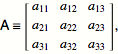
\includegraphics[width=1.5in]
{omitted-var-bias/3d-matrix.png}
\caption{Arbitrary 3 dimensional matrix $A$}
\label{fig-3dim-matrix}
\end{figure}

\begin{figure}[h!]
\centering
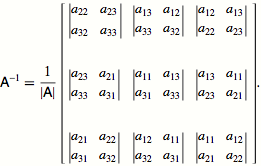
\includegraphics[width=3in]
{omitted-var-bias/3d-matrix-inv.png}
\caption{Inverse of 3 dimensional matrix $A$}
\label{fig-3dim-matrix-inv}
\end{figure}



